% ARTICLE 2 ----
% This is just here so I know exactly what I'm looking at in Rstudio when messing with stuff.
% Options for packages loaded elsewhere
\PassOptionsToPackage{unicode}{hyperref}
\PassOptionsToPackage{hyphens}{url}
%
\documentclass[
  11pt,
]{article}
\usepackage{lmodern}
\usepackage{amssymb,amsmath}
\usepackage{ifxetex,ifluatex}
\ifnum 0\ifxetex 1\fi\ifluatex 1\fi=0 % if pdftex
  \usepackage[T1]{fontenc}
  \usepackage[utf8]{inputenc}
  \usepackage{textcomp} % provide euro and other symbols
\else % if luatex or xetex
  \usepackage{unicode-math}
  \defaultfontfeatures{Scale=MatchLowercase}
  \defaultfontfeatures[\rmfamily]{Ligatures=TeX,Scale=1}
  \setmainfont[]{cochineal}
\fi
% Use upquote if available, for straight quotes in verbatim environments
\IfFileExists{upquote.sty}{\usepackage{upquote}}{}
\IfFileExists{microtype.sty}{% use microtype if available
  \usepackage[]{microtype}
  \UseMicrotypeSet[protrusion]{basicmath} % disable protrusion for tt fonts
}{}
\makeatletter
\@ifundefined{KOMAClassName}{% if non-KOMA class
  \IfFileExists{parskip.sty}{%
    \usepackage{parskip}
  }{% else
    \setlength{\parindent}{0pt}
    \setlength{\parskip}{6pt plus 2pt minus 1pt}
    }
}{% if KOMA class
  \KOMAoptions{parskip=half}}
\makeatother
\usepackage{xcolor}
\IfFileExists{xurl.sty}{\usepackage{xurl}}{} % add URL line breaks if available
\urlstyle{same} % disable monospaced font for URLs
\usepackage[margin=1in]{geometry}
\usepackage{graphicx}
\makeatletter
\def\maxwidth{\ifdim\Gin@nat@width>\linewidth\linewidth\else\Gin@nat@width\fi}
\def\maxheight{\ifdim\Gin@nat@height>\textheight\textheight\else\Gin@nat@height\fi}
\makeatother
% Scale images if necessary, so that they will not overflow the page
% margins by default, and it is still possible to overwrite the defaults
% using explicit options in \includegraphics[width, height, ...]{}
\setkeys{Gin}{width=\maxwidth,height=\maxheight,keepaspectratio}
% Set default figure placement to htbp
\makeatletter
\def\fps@figure{htbp}
\makeatother
\setlength{\emergencystretch}{3em} % prevent overfull lines
\providecommand{\tightlist}{%
  \setlength{\itemsep}{0pt}\setlength{\parskip}{0pt}}
\setcounter{secnumdepth}{-\maxdimen} % remove section numbering

\ifluatex
  \usepackage{selnolig}  % disable illegal ligatures
\fi
\usepackage[]{natbib}
\bibliographystyle{apsr}


\title{Fancy Paper Title Goes Here\thanks{Replication files are
available on the author's Github account (\url{http://github.com}).
\textbf{Current version}: May 09, 2022; \textbf{Corresponding author}:
\href{mailto:email@uni-mannheim.de}{\nolinkurl{email@uni-mannheim.de}}.}}
\author{true \and true}
\date{May 09, 2022}

% Jesus, okay, everything above this comment is default Pandoc LaTeX template. -----
% ----------------------------------------------------------------------------------
% I think I had assumed beamer and LaTex were somehow different templates.


\usepackage{kantlipsum}

\usepackage{abstract}
\renewcommand{\abstractname}{}    % clear the title
\renewcommand{\absnamepos}{empty} % originally center

\renewenvironment{abstract}
 {{%
    \setlength{\leftmargin}{0mm}
    \setlength{\rightmargin}{\leftmargin}%
  }%
  \relax}
 {\endlist}

\makeatletter
\def\@maketitle{%
  \newpage
%  \null
%  \vskip 2em%
%  \begin{center}%
  \let \footnote \thanks
      {\fontsize{18}{20}\selectfont\raggedright  \setlength{\parindent}{0pt} \@title \par}
    }
%\fi
\makeatother


\title{Fancy Paper Title Goes Here\thanks{Replication files are
available on the author's Github account (\url{http://github.com}).
\textbf{Current version}: May 09, 2022; \textbf{Corresponding author}:
\href{mailto:email@uni-mannheim.de}{\nolinkurl{email@uni-mannheim.de}}.}  }

\date{}

\usepackage{titlesec}

% 
\titleformat*{\section}{\large\bfseries}
\titleformat*{\subsection}{\normalsize\itshape} % \small\uppercase
\titleformat*{\subsubsection}{\normalsize\itshape}
\titleformat*{\paragraph}{\normalsize\itshape}
\titleformat*{\subparagraph}{\normalsize\itshape}

% add some other packages ----------

% \usepackage{multicol}
% This should regulate where figures float
% See: https://tex.stackexchange.com/questions/2275/keeping-tables-figures-close-to-where-they-are-mentioned
\usepackage[section]{placeins}



\makeatletter
\@ifpackageloaded{hyperref}{}{%
\ifxetex
  \PassOptionsToPackage{hyphens}{url}\usepackage[setpagesize=false, % page size defined by xetex
              unicode=false, % unicode breaks when used with xetex
              xetex]{hyperref}
\else
  \PassOptionsToPackage{hyphens}{url}\usepackage[draft,unicode=true]{hyperref}
\fi
}

\@ifpackageloaded{color}{
    \PassOptionsToPackage{usenames,dvipsnames}{color}
}{%
    \usepackage[usenames,dvipsnames]{color}
}
\makeatother
\hypersetup{breaklinks=true,
            bookmarks=true,
            pdfauthor={Carlos B. Gueiros (Universtität
Mannheim) and Marie-Therese Meye (Universtität Mannheim)},
             pdfkeywords = {inequality, social mobility, politics},
            pdftitle={Fancy Paper Title Goes Here},
            colorlinks=true,
            citecolor=blue,
            urlcolor=blue,
            linkcolor=magenta,
            pdfborder={0 0 0}}
\urlstyle{same}  % don't use monospace font for urls

% Add an option for endnotes. -----



% This will better treat References as a section when using natbib
% https://tex.stackexchange.com/questions/49962/bibliography-title-fontsize-problem-with-bibtex-and-the-natbib-package
\renewcommand\bibsection{%
   \section*{References}%
   \markboth{\MakeUppercase{\refname}}{\MakeUppercase{\refname}}%
  }%

% set default figure placement to htbp
\makeatletter
\def\fps@figure{htbp}
\makeatother



\usepackage{longtable}
\LTcapwidth=.95\textwidth
\linespread{1.05}
\usepackage{hyperref}

\newtheorem{hypothesis}{Hypothesis}


% trick for moving figures to back of document
% really wish we'd knock this shit off with moving tables/figures to back of document
% but, alas...

% 
% Optional code chunks ------
% SOURCE: https://stackoverflow.com/questions/50702942/does-rmarkdown-allow-captions-and-references-for-code-chunks



\begin{document}

% \textsf{\textbf{This is sans-serif bold text.}}
% \textbf{\textsf{This is bold sans-serif text.}}


% \maketitle

{% \usefont{T1}{pnc}{m}{n}
\setlength{\parindent}{0pt}
\thispagestyle{plain}
{%\fontsize{18}{20}\selectfont\raggedright
\maketitle  % title \par

}




{
   \vskip 13.5pt\relax \normalsize\fontsize{11}{12}
   \MakeUppercase{Carlos B. Gueiros}, \small{Universtität
Mannheim}   \par \vskip -3.5pt \MakeUppercase{Marie-Therese
Meye}, \small{Universtität Mannheim}   

}

}








\begin{abstract}

%    \hbox{\vrule height .2pt width 39.14pc}

    \vskip 8.5pt % \small

\noindent \small{Lorem ipsum dolor sit amet, consectetur adipiscing
elit. Donec sit amet libero justo. Pellentesque eget nibh ex. Aliquam
tincidunt egestas lectus id ullamcorper. Proin tellus orci, posuere sed
cursus at, bibendum ac odio. Nam consequat non ante eget aliquam. Nulla
facilisis tincidunt elit. Nunc hendrerit pellentesque quam, eu imperdiet
ipsum porttitor ut. Interdum et malesuada fames ac ante ipsum primis in
faucibus. Suspendisse potenti. Duis vitae nibh mauris. Duis nec sem sit
amet ante dictum mattis. Suspendisse diam velit, maximus eget commodo
at, faucibus et nisi. Ut a pellentesque eros, sit amet suscipit eros.
Nunc tincidunt quis risus suscipit vestibulum. Quisque eu fringilla
massa.}


\vskip 8.5pt \noindent \emph{Keywords}: inequality, social mobility,
politics \par

%    \hbox{\vrule height .2pt width 39.14pc}



\end{abstract}


\vskip -8.5pt


 % removetitleabstract


\setlength{\parindent}{16pt}
\setlength{\parskip}{0pt}

% We'll put doublespacing here
% Remember to cut it out later before bib
\hypertarget{introduction}{%
\section{Introduction}\label{introduction}}

Example of in text citation is \citet{king2001}, \ldots{}

Or you can cite like this \citep{king2001}.

\hypertarget{a-subsection-in-the-introduction}{%
\subsection{A Subsection in the
Introduction}\label{a-subsection-in-the-introduction}}

\kant[2]

\hypertarget{related-literature}{%
\section{Related Literature}\label{related-literature}}

\hypertarget{research-design}{%
\section{Research Design}\label{research-design}}

\hypertarget{data}{%
\subsection{Data}\label{data}}

\hypertarget{empirical-strategy-or-method}{%
\subsection{Empirical Strategy or
Method}\label{empirical-strategy-or-method}}

\hypertarget{results}{%
\section{Results}\label{results}}

\hypertarget{conclusion}{%
\section{Conclusion}\label{conclusion}}

\kant[24]

\hypertarget{including-plots}{%
\subsection{Including Plots}\label{including-plots}}

You can also embed plots, for example:

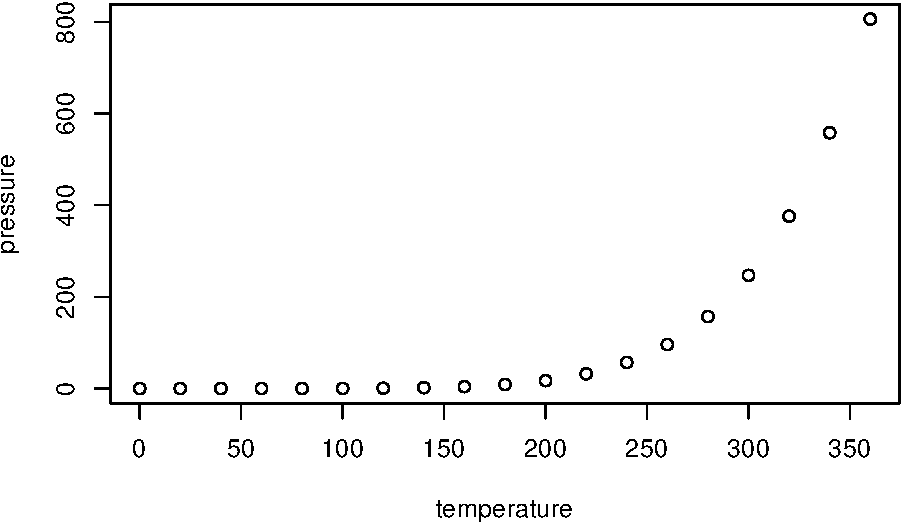
\includegraphics{paper_files/figure-latex/pressure-1.pdf}

\kant[25]

\renewcommand\refname{References}
  \bibliography{references.bib}


% should be about here.
% We'll put doublespacing end here

\end{document}
